\chapter{"Vault" Multisig Implementation}
\section{Multisig Smart Contract}
\label{ch4sec1}
In order to set up the multisig wallet, we have to create a smart contract that runs on the blockchain and complies into bytecode.  Let's examine each of the key components of a multisig smart contract:
\par 1. Storage Variables
\par The following are some important storage variables and their purposes in my specific contracts:
 \begin{itemize}
 	\item Owners: During deployment, an immutable list of addresses is initialized that lists the people who are allowed to communicate with the multisig instance.
 	\item numConfirmationsRequired: A number that specifies how many approvals transaction need to have until it can be executed.
 	\item Transactions:  A list of structures containing all relevant transaction data: value (in Ether), data, the destination address, and the current number of approvals.
 \end{itemize}
\par 2. View Functions
\par An essential component of Solidity are the view functions, which let you query data from smart contracts without altering their state.
\par Key Characteristics of view functions are:
 \begin{itemize}
	\item Do not alter state: View functions, in contrast to regular functions, are unable to alter contract state variables like storage or account balances.
	\item They don't require a transaction to be called directly by other smart contracts or online interfaces.
	\item Unlike functions that change states, calling them does not cost any gas
\end{itemize}
Some examples of the view functions used in the "Vault" Multisig Contract are: getOwners, getTransactions, getApprovedOwners (returns all the owners who approved a specific transaction)
\par 3. Regular Functions
\par Functions make it possible to manipulate data and carry out actions that change the contract's state, they are crucial to smart contracts. The key functions of the multisig contract are:
 \begin{itemize}
	\item submitTransaction(address \_to, uint256 \_value, bytes memory \_data): This is the first transaction you need to call in order to propose a transaction to be approved by the owners.
	\item confirmTransaction(uint256 \_txIndex):  An owner-specific call will be made to this function to authorize a transaction. Take note that nothing else is required—just the transaction ID. This is because you can determine which address started the transaction by accessing msg.sender.
	\item revokeConfirmation: This feature will revoke an approval.
	\item executeTransaction(uint256 \_txIndex): This function will finally carry out the transaction once the necessary number of confirmations has been received.
\end{itemize}
\par 3. Solidity Events
\par Solidity events are an important feature in the Solidity programming. They allow smart contracts to communicate with outside applications via "logs" that are stored in the blockchain \cite{soliditylogs}. They are very usefull because you can query them to see what transactions happend in the past but also listen to them in real time to update the interface in real time. Some logs this smart contract uses are: Deposit, SubmitTransaction, ConfirmTransaction, ExecuteTransaction. This events make it really usefull to query when any sort of action happend in the multisig contract

\section{Atlas - 2FA Feature}
\label{ch4sec2}
Atlas is a 6 digits one time password that you can set up for your multisig to provide additional security. It is a opt-in feature and you need to enable it yourself if you want to use it.
\par \textbf{How did I come up with this idea?}
\par Another blockchain called MultiversX, formerly known as Elrond, served as the model for Atlas. "Guardian" is the name of a comparable feature that MultiversX implemented. Any account can be configured with guardians to add further security. "The Great Heist" was arranged as an event to demonstrate the extra degree of security. The main goal of the event was to build up a wallet holding more than \$20,000. After the guardian was in place, the MultiversX team tweeted the account's mnemonic. Everyone was informed that the money will be retained by the first person to pass the guardian. But none was able to overcome it. This was an excellent example of the guardian OTP's security.
\par\textbf{How do One Time Passwords work (OTP)?}
\begin{figure}[htbp]
	\centering
	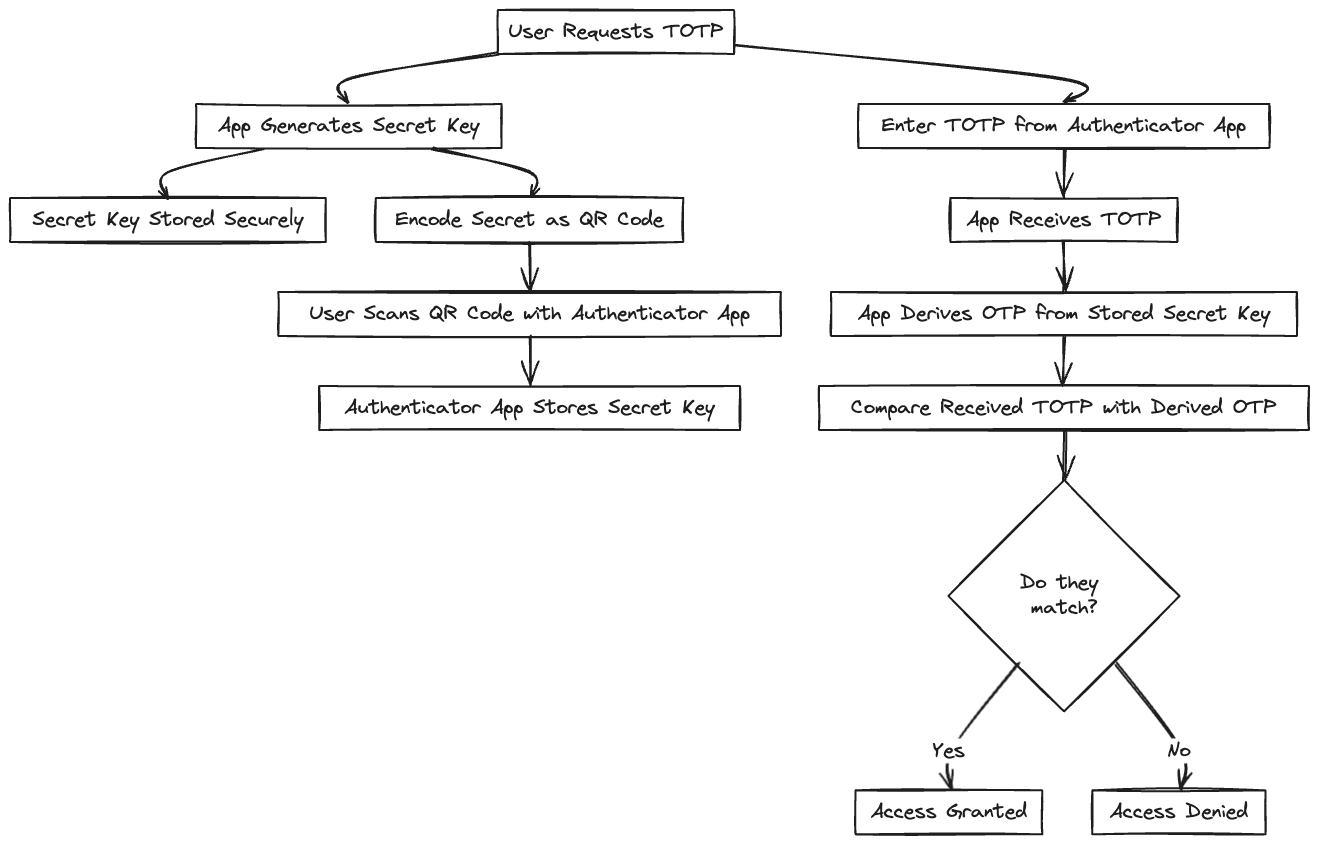
\includegraphics[scale=0.35]{./figures/totp.png}
	\caption{Generating and Validating OTPs}
\end{figure}
\par \textbf{Server side} 
A secret key, which is a string of alphanumeric characters, is created by the server and is specifically linked to the user's account. It generates a QR code with this secret key that mobile authenticator apps can use to set up the OTP.  Additionally, the server develops a function that will verify any OTP codes that are generated for that specific moment in time with the proper code that is received from the user.
\par \textbf{Client side} 
Using an authenticator app such as Google Authenticator, the user scans the given QR code. This app creates unique OTP codes by storing the secret key and using it in conjunction with the current time. Later, when they try to log into the online platform, the user enters the OTP code that the software created.
\par \textbf{OTP Validation Process} 
The user enters the OTP code from the authenticator app in addition to their standard password. The server then verifies that the password matches the one linked to the account and determines whether the provided OTP code is valid for the current time window. The user is granted access by the server if both the password and the OTP are verified. Successful verification depends on the server and the device issuing the OTP being in sync with one another in terms of time.  On the server, the secret key needs to be safely kept and protected from any potential unwanted access. To ensure reliability, standardized algorithms (TOTP or HOTP) should be used for OTP generation.
\par \textbf{How to implement Web3 OTP's} 
\par To use Atlas, you must first validate, first configure an OTP using an authenticator such as google authenticator. After the authenticator has been activated and validated, the server will remember the private key that corresponds to the multisig wallet address. To activate the otp on chain, the server will send you the etherum address corresponding to the private key with which the otp is generated to the client, and the client will "propose" an Atlas activation by calling the endpoint: proposeAtlasActivation(address \_atlasAddress). For any change of the atlas a timeout period is implemented, we will talk about it below. After the timeout has passed, the activateAtlas() endpoint can be called to activate Atlas, and consequently no transaction from now on will be able to be approved without validating the OTP code. If somehow the user loses access to the used authenticator, he could propose a deactivation of atlas, which will also be subject to the same timeout period, until it can be permanently deactivated.

\par \textbf{How does Atlas help?} 
\par In the unlikely event that your private key is obtained by an adversary, Atlas comes in quite handy. In this instance, if Atlas was enabled, he would not have been able to take money out of your account without also verifying Atlas. In this instance, the thief must first disable the atlas, which is governed by the previously stated timeout duration. During this period, the account holder will be able to move all of the money to a different address and prevent any money from being stolen because they will have access to both the private key and the OTP.
\par \textbf{First Attempt: Confirming Atlas on the server}
\par My first attempt was to set up a POST request on my server that would validate the OTP for a certain multisig wallet. If the otp was correct the server would sign a transaction with the private key that generated this otp and send this transaction to the multisig contract. However this has a major setback. For the account generated with the OTP private key to interact with the multisig contract this would need to have Ether in it to cover the transaction fees. I decided that this approch is not optimal because it is very user unfriendly. The user should not know that atlas is actually another account that needs to be constantly be topped up to work.
\par \textbf{Second Attempt: Sending a signed message to the client}
\par After thinking a bit how to not make the private key on the server cover the transaction fees on the server I finally came up with a solution that I think its much better. The solution was changing the multisig contract. At first the confirmAtlas endpoint had just one parameter, the id of the transaction the user would want Atlas to confirm it. Moreover the confirmAtlas could only be called by the address generated from the private key of the otp. After the modification the confirmAtlas still had the id of the transaction, but it also had an additional parameter named "signature". The solution I found was to sign the id of the transaction the user would want to confirm on the server and than return it to the client. The client would call the confirmAtlas endpoint with the index, and the signature and the smart contract would validate that this signed message was signed by the private key of the atlas account. The code looks like this:
\newline
\begin{verbatim}
function confirmAtlas(
	uint256 _txIndex, 
	bytes memory signature
) public {
		require(atlasAddress != address(0), "Atlas not activated");
		require(_txIndex < transactions.length, "tx does not exist");
		Transaction storage transaction = transactions[_txIndex];
		require(!transaction.atlasConfirmed, "Atlas already confirmed");
			
		bytes32 messageHash = keccak256(abi.encodePacked(_txIndex));
		bytes32 ethSignedMessageHash = keccak256(
		abi.encodePacked("\x19Ethereum Signed Message:\n32", messageHash));
			
		(address recoveredAddress) = recoverSigner(ethSignedMessageHash, signature);
		require(recoveredAddress == atlasAddress, "Invalid signature");
				
		transaction.atlasConfirmed = true;
}
\end{verbatim}
%\newline
This is a major improvement because now the atlas account does not need to have any ether in it so that it can approve a transaction
\par \textbf{Common Questions}
\par 1. What occurs if someone steals the Atlas Private key? Should that prove to be true, there wouldn't be a significant security issue. The Atlas private key is limited to approving transactions; it cannot initiate new transactions or communicate in any manner with the multisig contract.
\par 2. Is the Atlas feature centralized? Yes, all the private keys are stored in a postgres database, nevertheless, this is not a security risk, as was mentioned in response to the initial question. Furthermore, you have the option to turn off the Atlas feature and continue using your account normally in the unlikely case that this third-party service stops functioning.

\section{Backend}
\label{ch4sec3}
Because most of the logic is handled by the multig smart contract I did not have to implement a lot of functionalities on the backend. Smart contracts can automate a large portion of business logic, particularly that which involves safe and verifiable transactions or interactions. They use the blockchain directly to carry out actions in an immutable and transparent manner. Many of the procedures that were needed to communicate constantly with a backend server are now decentralized thanks to smart contracts. This lessens potential points of failure and attacks that could interfere with the application's ability to function. In an application for a multisig account the smart contract handles 90\% of the logic. The only need for the backend was to store the private keys for the Atlas feature and to cache some information to not make a lot of request to the Infura API.
\par\textbf{Why NextJS?}
For my project's backend, I decided to use Next.js for a few reasons. Firstly, Next.js provides amazing ability when it comes to content rendering. By sending pages fast and effectively, entities may maximize speed and user experience with Server-Side Rendering (SSR) and Static Generation (SSG) choices. For my applications, where quick interactions and real-time data display are crucial this is necessary. I can manage backend logic using serverless functions instead of constantly operating a typical server thanks to Next.js. This implies that they are able to manage dynamic requests and interactions with the database or other APIs in a manner that is more economical and efficient. Scalability becomes easier because functions are only called upon when necessary, preventing resource waste and the related expenses of a server operating constantly.
\par For the Atlas feature instead of using http routes I mostly used "Server Actions". Server actions makes it very easy to write functions that are executed in the server in the same project where your frontend is located. This is an example of a server function and how it looks like:

\begin{verbatim}
"use server"
export const getConfirmAtlasSignature = async (
		otp: string,
		txIndex: number,
		multisigAddress: string,
		chain: number
) => {
		const isValid = checkOTP(otp, multisigAddress);
		if (!isValid) {
			throw new Error("Invalid OTP");
		}
		const wallet = (
		await db
		.select()
		.from(WalletsTable)
		.where(sql`${WalletsTable.walletAddress} = ${multisigAddress}`)
		)[0];
		if (!wallet.secret) {
			throw new Error("Secret not found");
		}
		if (!wallet.atlasAddress) {
			throw new Error("Atlas address not found");
		}
		const hexSecret = Buffer.from(
		base32Decode(wallet.secret, "RFC4648")
		).toString("hex");
		const provider = new ethers.InfuraProvider(
		chain,
		"b3615957c6b0427eb2fac15afb451acb"
		);
		const signer = new ethers.Wallet(hexSecret, provider);
		const messageHash = ethers.solidityPackedKeccak256(["uint256"], [txIndex]);
		const messageBytes = ethers.getBytes(messageHash);
		const signature = await signer.signMessage(messageBytes);
		return signature;
};
\end{verbatim}

As it can be seen the "use server" expression indicates that the functions declared in the file will only be used on the server, as can be observed. This causes the function to retrieve data or perform updates on it from sources such as the Postgres database. This function can be used directly in a button onclick handler and nextjs will handle the comunication. 
\par The provided function is also how the Atlas confirmation is implemented on the backend. This is how it works
\begin{enumerate}
\item Verify OTP: The function begins by determining whether the user-provided one-time password (OTP) is valid. In order to verify that the individual attempting to complete a sensitive activity or execute a transaction is, in fact, the authorized user, this check is crucial for the 2FA functionality. An error is raised right away if the OTP is invalid.
\item Retrieve Wallet Information: The function then goes on to obtain wallet data from a database. It precisely looks for a wallet that corresponds to the given multisigAddress. This address usually refers to a multi-signature wallet, which increases security by requiring multiple keys to allow transactions. Errors are raised appropriately if the wallet lacks linked secret keys or an Atlas address.
\item Decode Secret Key: The base32-formatted secret linked to the wallet is subsequently converted to hexadecimal. The secret key must be in a certain format for the subsequent cryptographic procedures, which makes this conversion required.
\item Create Blockchain Provider and Signer: This function uses Infura and Ethers.js to create a blockchain provider. Using Infura, you can interact with the Ethereum blockchain without having to manage your own node by using their scalable blockchain node network. To generate a new Ethereum wallet instance (signer) that may sign messages or transactions, utilize the decrypted secret key.
\item Get the message ready to sign: The transaction index (txIndex) is hashed using a technique that works with Solidity, the Ethereum smart contract language. This guarantees that the hash can be replicated and validated on the blockchain and establishes a common method for encoding different kinds of data.
\item Put the atlas signature on the message: After that, the transaction index hash is translated to bytes, and the byte data is signed by the Ethereum wallet instance. When data is signed, a cryptographic signature is created that can be checked on the blockchain to confirm that the signer—the owner of the private key linked to the multisigAddress—signed the document.
\item Give the signature back: Ultimately, this signature is returned by the function. This signature acts as a cryptographic demonstration that the user has the private key linked to the wallet and that they have verified their identity using the proper OTP. 
\end{enumerate}
\section{Database}
\label{ch4sec4}
I choose PostgreSQL as the database for my project mostly because of its reliability and capacity to manage secure transactions and complex search functions well. For applications that demand a high degree of security and dependability, PostgreSQL is known for complying to ACID standards, which ensures dependable transactions and consistent data integrity. Another important reason for wich i chose Postgres is because I had experience working with it.
\par Yet the PostgreSQL database structure in this project is very minimal, and this choice is directly tied to the fact that a large portion of the  logic is implemented using smart contracts on the blockchain. By storing data and transactions directly on the blockchain through smart contracts, it can decentralize important activities and cut down on the need to use the database for the same things. For instance, blockchain is used to monitor and verify information about user transactions, contract statuses, and other important data, increasing security and transparency.
\par This means that the PostgreSQL database is used more for storing auxiliary data that does not require the same level of security or is not directly related to the logic of the smart contract. In this instance, all of the multisig wallets we've created on this platform are stored in the postgres database for quick access. This data is additionally on the blockchain, but we can store it in a database rather than continually searching the network once a wallet is configured and stops chaining. Database scalability is aided. It can also hold other data, such as user profile details like names, emails, preferred themes, and so forth, that is not included in the blockchain.
\section{Frontend}
\label{ch4sec5}
\par For the frontend portion of the project, I decided to use Next.js due to a number of significant benefits this framework provides. I can use reusable components and state management to create a responsive and fluid user experience since Next.js integrates with React easily and is incredibly effective at creating modern, dynamic user interfaces.
\par The fact that Next.js can implement server-side rendering (SSR) and static site generation (SSG) is one of the key reasons I chose it. The information is pre-rendered and ready to be supplied to users and search engines, which enables me to optimize the application's performance and improve SEO and page load speeds. React server components allow for the direct fetching of data and waiting on it. As I mentioned before, this improves user experience and speeds up loading times by allowing viewers to see all of the data rather than just spinning images. 

\par Additionally, Next.js has code optimization and automatic routing right out of the box, which cuts down on development time and the difficulty of maintaining dependencies and routes. These capabilities free me up from the minutiae of configuration and optimization so that I can concentrate more on creating application-specific functionality.

\par \textbf{Folder Structure}
\par The project uses a scalable folder structure in this project. I store all publicly accessible static resources (such photos, fonts, and favicon files) that may be directly referenced in code under the public directory.
\par The project's main section, the src directory, here are the following folders located:
\begin{itemize}
	\item \textbf{app}: The Next.js project's app directory file structure is used by the App Router to directly define routes. Consider a file called app/page, for instance.The root route (/) naturally correlates to page.ts. Inside this folder you can also put different files like layout.ts, error.ts or loading.ts to handle different things like loading animations or error boundries.
	\item \textbf{components}: The components directory contains reusable React components for building the user interface. There are several components directories in other folders to organize components specific to each domain of the application, the top components directory is only used to store components that are used everywhere in the application
	\item \textbf{contracts}: The contracts directory is used to store contracts that are going to be used in the app like the multisig contract. It stores the contract ABI to make typescript understand how it can interact with the contract and make the development typesafe. It also stores the bytecode of the contract so the app can deploy instances of it.
	\item \textbf{db}: This directory contains everything related to database interactions, including configuration scripts, data models, and any other utilities needed to manipulate data.
	\item \textbf{helpers}: Utility functions that are utilized throughout the project are stored in the helpers directory. These aspects encourage the reuse of logic and prevent code duplication. The difference between the helpers and the lib directory is that the helpers does not contain any businiss logic specifically for this project.
	\item \textbf{hooks}: This is where React's custom hooks are placed, which allow state logic to be extracted and reused in components. This improves modularity, testability, readability and maintainablility.
	\item \textbf{lib}: The lib directory (short for "library") is used to store code that handles business logic or complex interactions in the application. For this project it is used to house the logic of the multisig and OTP.
	\item \textbf{service}: Services that manipulate data or perform specific operations are implemented in the service directory, acting as intermediaries between other apis or databases.
	\item \textbf{types}: this directory is used to define custom TypeScript types that are used to ensure correct typing within the project
	\item \textbf{validations}: This directory contains validation schemes necessary to ensure that the data entered into the application is correct and complete
\end{itemize}
\par \textbf{Styling and building Reusable Components}
\par I chose to use Tailwind CSS for its efficiency and flexibility. Tailwind provides utility classes that allow quick and direct HTML customization. This increases development speed and eliminates the need to write additional CSS code. Using granular design control, Tailwind helped me build responsive and custom interfaces with minimal effort. It was also extremely helpful in maintaining style consistency throughout the application. 
\par Because it takes a lot of time to build components from scratch, I decided to use the NextUi and Shadcn UI libraries. Because you can import certain components, like buttons or modals, and not the complete library to use it, I choose to use two libraries. For instance, I utilized the modals from nextUi because I prefer their animations and they are more responsive for mobile devices, and I used the buttons from shadcn since they are much more simple. 
\par \textbf{Project Pages}
This are the folowing pages that are used inside the application:
\begin{itemize}
	\item \textbf{Create Wallet}: This is the first page a new user sees. Here you can choose the chain, create a new multisig wallet, select the owners and the number of signatures required to approve a transaction
	\item \textbf{Select Wallet}: The page provides an interface to select one of the existing multisig wallets. It is useful for quickly switching between wallets.
	\item \textbf{Dashboard}: Here, users can see an overview of the selected wallet, including balance and other relevant metrics. It also provides quick access to frequently used functions, such as initiating a transaction or viewing your transaction history.
	\item \textbf{Atlas Page}: This is the page where you can setup your Atlas 2FA. This page has different states. One of the states is if atlas is not configured you can set it up with your authenticator. Another one is if Atlas is configured, than you can see details such as the atlas address.
	\item \textbf{Transactions}: This page lists all transactions made or proposed in the multisig wallet. Users can see a preview of how many owners have accepted the transaction as well as the history of all transactions that were initiated by this multisig.
	\item \textbf{Transaction Details}: You may view every detail of a particular transaction right here. The data field, value, transaction id, and transaction hash. If you are the owner, you can also validate Atlas and carry out the transaction if you have enough approvals. You can also approve or reject the transaction.
\end{itemize}
